
% \documentclass[notes=show]{beamer}
\documentclass[xcolor=dvipsnames, xcolor=table, 10pt]{beamer}
%%%%%%%%%%%%%%%%%%%%%%%%%%%%%%%%%%%%%%%%%%%%%%%%%%%%%%%%%%%%%%%%%%%%%%%%%%%%%%%%%%%%%%%%%%%%%%%%%%%%%%%%%%%%%%%%%%%%%%%%%%%%%%%%%%%%%%%%%%%%%%%%%%%%%%%%%%%%%%%%%%%%%%%%%%%%%%%%%%%%%%%%%%%%%%%%%%%%%%%%%%%%%%%%%%%%%%%%%%%%%%%%%%%%%%%%%%%%%%%%%%%%%%%%%%%%

\usepackage{amsmath}
\usepackage{mathpazo}
\usepackage[authoryear]{natbib}             % Option: Use NatBib bibliography styles
\usepackage{hyperref}
\usepackage{multimedia}
\usepackage{graphicx}
\usepackage{helvet}
\usepackage[english]{babel}
\usepackage[latin1]{inputenc}
\usepackage{comment}
\usepackage{color}
\usepackage{epstopdf}
\usepackage{appendixnumberbeamer}
\usepackage{transparent}
\usepackage{xcolor}
\usepackage{relsize}
\usepackage{booktabs}
\usepackage{amsthm}
\usepackage{threeparttable, tablefootnote} % table footnote
\usepackage{PlayfairDisplay}

\DeclareMathOperator*{\argmin}{argmin} % thin space, limits underneath in displays
\usepackage{bbm}



\setcounter{MaxMatrixCols}{10}

% \useinnertheme{circles}
\usefonttheme{serif}
% \usecolortheme{orchid}

\usecolortheme[RGB={26,58,95}]{structure}
\beamertemplatenavigationsymbolsempty

\definecolor{orange}{RGB}{255,127,0}
\newcommand{\bb}[1]{{\color{euiblue}#1}}
\newcommand{\gre}[1]{{\color{applegreen}#1}}
\newcommand{\rr}[1]{{\color{darkred}#1}}
\newcommand{\orr}[1]{{\color{orange}#1}}
\definecolor{upf}{RGB}{192,0,37}
\definecolor{euiblue}{RGB}{56,136,199}
\definecolor{fedblue}{RGB}{26,58,95}
\definecolor{darkred}{rgb}{0.55, 0.0, 0.0}
\definecolor{applegreen}{rgb}{0.55, 0.71, 0.0}
\definecolor{orange}{rgb}{0.93, 0.53, 0.18}

\usepackage{mathtools}

 \newcommand{\lefta}{ \left[\begin{array} } 	
\newcommand{\righta}{ \end{array} \right]} 	

\newcommand*{\vcenterimage}[1]{\vcenter{\hbox{\includegraphics[width=0.35\linewidth]{#1}}}}
\newcommand*{\vcenterarrow}{\vcenter{\hbox{$\Longrightarrow$}}}

\makeatletter
\def\blfootnote{\gdef\@thefnmark{}\@footnotetext}
\makeatother


\useitemizeitemtemplate{%
    \raise1.5pt\hbox{\color{beamerstructure}$\bullet$}%
}
\usesubitemizeitemtemplate{%
    \small\raise1.5pt\hbox{\color{beamerstructure}$\bullet$}%
}
\usesubsubitemizeitemtemplate{%
    \raise1.5pt\hbox{\color{beamerstructure}$\circ$}%
}


\setbeamersize{text margin left=1.5em,text margin right=1.5em}
\setbeamertemplate{footline}[frame number]

\usetheme{boadilla}


\begin{document}

\playfair

\title[Understanding Growth at Risk]{\textbf{Understanding Growth at Risk}}
\thispagestyle{empty}
\author[Caldara, Cascaldi-Garcia, Cuba Borda, Loria]{\textbf{Dario Caldara (IF)\\ Danilo Cascaldi-Garcia (IF)\\ Pablo Cuba Borda (IF)\\ Francesca Loria (R\&S)}\\ \emph{Board of Governors of the Federal Reserve System}}

%\date[Class II - FOMC]{\emph{May 12, 2020}}
\date[Nonconfidential External]{\emph{May 12, 2020}}

\maketitle

% \begin{frame}{Overview}
% \tableofcontents
% \end{frame}

\setcounter{framenumber}{0}
\begin{frame}{An Overview of ``Growth-at-Risk"}
\vspace*{0.12in}
\begin{itemize}
    \item {\bb{Goal:}} Measure uncertainty and risks around forecast.
    \bigskip    
    \item Model the \rr{entire} distribution of future real GDP growth \rr{conditional on economic activity and financial conditions}.
    \bigskip
    \item Key result: (Conditional) mean and volatility are negatively correlated.\\    
    \begin{center}
        $\longrightarrow$ \rr{Growth-at-Risk}! 
    \end{center}
    % \medskip
    
    %     \begin{itemize}
    %         \item {\footnotesize High mean - Low volatility: Normal state}
    %         \medskip
    %         \item {\footnotesize Low mean - High volatility: Large downside risks} 
    %    \end{itemize}
\end{itemize}
\begin{figure}
    \includegraphics[width=0.85\linewidth,keepaspectratio=true]{Figures/univariatefull-VC.pdf}
\end{figure}

\end{frame}

% \begin{frame}{Modelling "Growth-at-Risk"}

% \begin{itemize}
%     \item GaR as negative correlation between mean and volatility is a very robust finding across modelling approaches:
%     \smallskip
%       \begin{enumerate}
%             \item \rr{Quantile regressions} (QR)
%             \medskip
%             \item \rr{Stochastic volatility VARs}
%             \medskip
%             \item Markov switching models
%             \medskip
%             \item  Conditionally heteroskedastic models
%         \end{enumerate}
%         \bigskip
%     \item Approaches vary in:
%     \smallskip
%         \begin{itemize}
%             \item Flexibility
%             \medskip
%             \item Robustness
%             \medskip
%             \item Computational burden
%             \medskip
%             \item Details of the results
%         \end{itemize}
% \end{itemize}

% \end{frame}

\begin{frame}{Plan of the Talk}

\begin{enumerate}
    \item Quantile Regressions
    \begin{enumerate}
    \smallskip
        \item Basic framework
        % \medskip
        % \item Times series of conditional quantiles
        \medskip
        \item Advantages and Disadvantages
        \medskip
        \item From Quantiles to Distributions
    \end{enumerate}
    \bigskip
    \item From Quantiles to Distributions
    \begin{enumerate}
    \smallskip
        \item Intuition
        \medskip
        \item Examples from 'real-time tracking of risks' \& 'inflation at risk'
        \medskip
    \end{enumerate}
\end{enumerate}

\end{frame}



\frame{
\frametitle{Fixing Ideas}
\vspace{0.25cm}

\begin{itemize}
\item Consider a variable $y_t$, with cumulative distribution function $F(y)$.
\item Conditional quantile function (CQF) of $y$ is
\begin{equation*}
  \text{Q}_{\tau} (y) = F^{-1}_y\left(\tau\right),\ \tau \in (0,1).
\end{equation*}

\begin{figure}[h!]
\includegraphics[width=0.6\textwidth]{Figures/CDF}
\end{figure}

\end{itemize}
}


\frame{
\frametitle{Conditional Quantiles}

\vspace{0.25cm}

\begin{itemize}
\item Quantile regression (QR):
\medskip
\begin{itemize}
\item Minimum mean squared error (MMSE) \textbf{linear approximation to the CQF}.
\medskip
\item Provides parametric linear model for $\text{Q}_{\tau} (y)$ $\Longrightarrow \text{Q}_{\tau} (y|x)=x \theta_{\tau}$.
\medskip
\item Allows to study relationship between quantiles and covariates $x$.

\begin{figure}[h!]
\includegraphics[width=0.6\textwidth]{Figures/CDF_QR}
\end{figure}


\end{itemize}
\end{itemize}
}


\frame{
\frametitle{Quantile Regressions}
\label{qr}
\vspace{0.25cm}

{\small
\begin{itemize}
\item Linear model for conditional quantile function
\begin{equation*}
\text{Q}_{\tau} (y_t| x_t) = x_t \theta_{\tau},\ \tau \in (0,1)
\end{equation*}
where quantile regression slopes solve
\begin{equation*}
\hspace{-0.2cm}  \theta_{\tau} = \argmin_{\theta_{\tau}\in\mathbb{R}^k} \sum_{t=1}^{T} \bigl[\rho_{\tau} \underbrace{\left(y_t -x_t \hat{\theta}_{\tau}\right)}_{\equiv u_t} \bigr]
\end{equation*}
and $\rho_{\tau}(u)= \mathbb{1}(u\leq 0) (1-\tau) u + \mathbb{1} (u >0) \tau u$ is the \hyperlink{checkfct}{\beamerbutton{Check Function}}.

\bigskip
\item Quantile regression \textbf{differs from OLS} in these dimensions:\medskip
\begin{enumerate}
	\item Minimizes the \emph{weighted} sum of \emph{absolute} (vs. squared) errors.\medskip
	\item Weights depend on error terms being above or below a quantile $\tau$.
\end{enumerate}
\bigskip
  \item \textbf{Example} of linear relationship between quantiles and conditioning variables:
\begin{equation*}
  \hat{\text{Q}}_{\tau} (\Delta \bar{y}_{t+1,t+12}| x_t) = \hat{\alpha}_{\tau} + \hat{\beta}_{\tau} VXO_t + \hat{\gamma}_{\tau} ADS_t,\ \tau \in (0,1).
\end{equation*}

\end{itemize}
}
}




% \section{Identification}
% \begin{frame}[noframenumbering]
% \thispagestyle{empty}
%       \begin{center}
%          \structure{\Huge {\color{black}{\insertsection}}}
%       \end{center}
%      \end{frame}

\frame{
\frametitle{Obtaining the Time Series of Conditional Quantiles}
\label{linearqr}
\vspace*{0.1in}
\begin{figure}[h!]
{\scriptsize{Note: Black circles indicate observations pairs after December 2007.}}
\includegraphics[width=0.45\textwidth]{Figures/slope_vix___Country=US___GDP=GDP___SpecWith=vix_ads___Scenario=Baseline___Lags=0___Sample=1986-Jan_to_2020-Mar}
 \includegraphics[width=0.45\textwidth]{Figures/slope_ads___Country=US___GDP=GDP___SpecWith=vix_ads___Scenario=Baseline___Lags=0___Sample=1986-Jan_to_2020-Mar}
\end{figure}

\begin{itemize}
    \item \textbf{Key takeaways}:
    \medskip
    \begin{enumerate}
        \item OLS and median are different (asymmetry).
        \medskip
        \item VXO and ADS stronger effect in lower quantiles\\ $\longrightarrow$\rr{Rise in volatility and skewness of GDP}.
    \end{enumerate}
 
\end{itemize}
\hyperlink{Data}{\beamerbutton{Data \& Estimation}}
\hyperlink{TSQSteps}{\beamerbutton{Fitted Values over Time}}

}


% \frame{
% \frametitle{Quantile Regression Slopes}
% \framesubtitle{From 'Growth At Risk Models for the U.S. and the Foreign Economy (2020)' }

% \begin{figure}[h!]
% {\scriptsize{Note: Black circles indicate observations pairs after December 2007.}}
% \includegraphics[width=0.49\textwidth]{Figures/slope_vix___Country=US___GDP=GDP___SpecWith=vix_ads___Scenario=Baseline___Lags=0___Sample=1986-Jan_to_2020-Mar}
%  \includegraphics[width=0.49\textwidth]{Figures/slope_ads___Country=US___GDP=GDP___SpecWith=vix_ads___Scenario=Baseline___Lags=0___Sample=1986-Jan_to_2020-Mar}
% \end{figure}

% \medskip

% \begin{itemize}
%     \item \textbf{Key takeaways}:
%     \medskip
%     \begin{enumerate}
%         \item OLS and median are different (asymmetry).
%         \medskip
%         \item Effect of VXO and ADS stronger in lower quantiles\\ $\longrightarrow$\alert{Rise in volatility and skewness of GDP}.
%     \end{enumerate}
% \end{itemize}
% }

% \frame{
% \frametitle{Quantile Regression Slopes\\ \small Economic Activity Index (ADS)}


% }



% \section{Quantiles over Time}
% \begin{frame}[noframenumbering]
% \thispagestyle{empty}
%       \begin{center}
%          \structure{\Huge {\color{black}{\insertsection}}}
%       \end{center}
%      \end{frame}

\frame{
\frametitle{Conditional Quantiles over Time}
\framesubtitle{From 'Growth At Risk Models for the U.S. and the Foreign Economy'\\ Caldara, Cascaldi-Garcia and Loria (2020)}
\begin{figure}[!htb]
 \centering
 \includegraphics[width=\textwidth]{Figures/quantilesfan_azzalini____Country=US___GDP=GDP___SpecWith=vix_ads___Scenario=Baseline___Lags=0___Detrended=true___Sample=1986-Jan_to_2020-Mar}
\end{figure}
}

\frame{
\frametitle{Conditional Quantiles over Time}
\framesubtitle{Assessing Statistical Significance \hyperlink{bootstrap}{\beamerbutton{Bootstrap}}}
\label{bootfullsample}
\begin{figure}[!htb]
 \centering
 \includegraphics[width=\textwidth]{Figures/quantiles_bootstrap}
\end{figure}
\hyperlink{bootGFC}{\beamerbutton{Global Financial Crisis}} \hyperlink{bootCOVID}{\beamerbutton{COVID-19}}
}

\frame{
\frametitle{Advantages and Disadvantages of QR}
\label{disadvantagesqr}
\begin{itemize}
    \item \textbf{Key advantages}:
    \medskip
       \begin{enumerate}
            \item Ease of implementation
            \medskip
            \item Distribution agnostic
            %\medskip
            %\item Robust to outliers
            \medskip
            \item Local approximations to more complex nonlinear models.
           % \item Ability to capture nonlinear effects.
        \end{enumerate}
        \bigskip
    \item \textbf{Disadvantages}:
    \medskip
        \begin{enumerate}
            \item Needs sufficient data.
            \medskip            
            \item Lower/upper quantile estimates can be less robust than mean \hyperlink{qr-estimates-abg}{\beamerbutton{ABG Example}}.
            % \rr{Example}. Staff has found that in financial stability applications:
            % \smallskip
            % \begin{itemize}
            %     \item Conditioning variables matter. \hyperlink{qr-estimates-abg}{\beamerbutton{ABG Example}}
            %     \smallskip
            %     \item Hard to generalize across countries.
            % \end{itemize}
            \medskip
            \item Local approximation only valid over region of interest. 
            % If approximation is poor then QR will suggest ``crossings'' of conditional quantiles.
        \end{enumerate}
\end{itemize}
}



% \section{From Quantiles to Distributions}
% \begin{frame}[noframenumbering]
% \thispagestyle{empty}
%       \begin{center}
%          \structure{\Huge {\color{black}{\insertsection}}}
%       \end{center}
%      \end{frame}



\frame{
\frametitle{From Estimated Quantiles to Distributions}
\label{azzintro}
\begin{itemize}
  \item \citet{Adrianetal2019}: Map estimated conditional quantiles into a probability distribution function (PDF).
  \bigskip
  \item \bb{Advantages}: Visualize shape of distribution, compute moments and statistics (e.g., 'recession' probabilities).
 \bigskip
  \item \rr{Disadvantages}: Ignores estimation uncertainty from QR, introduces approximation error \hyperlink{approxerrorabg}{\beamerbutton{ABG Illustration}}.
\bigskip
  \item \gre{Approach}: Smooth quantile function using the skewed $t-$distribution of \citet{AzzaliniCapitanio} characterized by four parameters:\\ {\begin{center} $\Theta$=(location, scale, skewness, kurtosis) \end{center}}
  \bigskip
  \item At each time $t$, minimize squared distance between conditional quantiles from QR model and quantiles implied by skewed $t-$PDF:
  \begin{center}
  \textit{Four quantiles to match four parameters.}
  \end{center}
\end{itemize}
\smallskip
\hyperlink{azzsbs}{\beamerbutton{Step-by-Step Example}} \hyperlink{PITs}{\beamerbutton{PITs}}
}


\frame{
\frametitle{Fitted Predictive Densities}
\framesubtitle{From 'Growth At Risk Models for the U.S. and the Foreign Economy'\\ Caldara, Cascaldi-Garcia and Loria (2020)}

\begin{figure}[!htb]
 \centering
 \includegraphics[width=0.9\textwidth]{Figures/pdf_IS___Country=US___GDP=GDP___SpecWith=vix_ads___Scenario=Baseline___Lags=0___Detrended=true___Sample=1986-Jan_to_2020-Mar}
\end{figure}

\begin{itemize}
  \item Decline in mean and rise in volatility.
  \medskip
  \item {\rr{Sharp rise in skewness}} (recurring finding in QR-Azzalini framework). 
\end{itemize}

}


\frame{
\frametitle{Inflation at Risk}
\framesubtitle{\citet{LSL20}}
\vspace{0.5cm}
\begin{itemize}
  \item Augmented Phillips-curve model with credit (financial) conditions:
  {\small
  \begin{equation*}
\widehat{\text{Q}}_{\tau}(\bar{\pi}_{t+1,t+12}|x_t) = (1 - \hat{\lambda}_{\tau}) \pi^*_{t-1} + \hat{\lambda}_{\tau} \pi^{LTE}_{t} + \hat{\theta}_{\tau} (u_t - u^*_t) +  \hat{\gamma}_{\tau} (\pi^R_t - \pi_t) + \rr{\hat{\delta}_{\tau} cs_t}\smallskip
\end{equation*}}

  \item Tight financial conditions (high credit spreads) carry substantial downside inflation risks and generate sharp rise in skewness. 
\end{itemize}
\bigskip
\begin{figure}[!htb]
 \centering
 \includegraphics[width=0.9\textwidth]{Figures/pdf___SpecWith=ugap_pistar_pO_pLTE_gzs___Sample=2000-Jan_to_2020-Mar.pdf}
\end{figure}

}


%%%%%%%%%%%
% APPENDIX
\appendix


% This sets the page counter back to 1:
\setcounter{framenumber}{0}
% And this makes LaTeX include the letter "A" in the page numbering
\renewcommand{\insertframenumber}{A-\arabic{framenumber}}
\renewcommand{\theframenumber}{A-\arabic{framenumber}}


\section{Appendix}
\begin{frame}[noframenumbering]
\thispagestyle{empty}
       \begin{center}
         \structure{\Huge {\color{black}{\insertsection}}}
       \end{center}
     \end{frame}
     


% \frame{
% \frametitle{Quantile Regression vs. Ordinary Least Squares}

% Quantile regression differs from OLS in these dimensions:\medskip
% \begin{enumerate}
% 	\item Minimizes the \emph{weighted} sum of \emph{absolute} (vs. squared) errors.\medskip
% 	\item Weights depend on error terms being above or below a quantile $\tau$.
% \end{enumerate}
% \bigskip
% \begin{figure}[!htb]
%  \centering
%  \includegraphics[width=\linewidth]{Figures/quantile_reg_comp}
%  \vspace{-0.25cm}
% {\tiny{Source: ``Five Things You Should Know about Quantile Regression'' by Rodriguez and Yao (2017).}}
% \end{figure}
% \vspace{-1.25cm}
% }



% \frame{
% \frametitle{The Flexibility of Quantile Regression Models}

% \begin{itemize}
%   \item Some notes on DGPs that they can approximate. (TBA)
%   \bigskip
%   \item \citet{KX2006}:
%   \medskip
%     \begin{itemize}
%         \item[--] Quantile regressions can capture the effects of the conditioning variables on the location, scale and shape of the conditional distribution of the response variable.
%             \medskip
%         \item[--] Significant extension of classical constant coefficient linear time series models in which the effect of conditioning is confined to a location shift.
%     \end{itemize}
% \end{itemize}
% }




\section{Check Function}
\begin{frame}[noframenumbering]
\thispagestyle{empty}
       \begin{center}
         \structure{\Huge {\color{black}{\insertsection}}}
       \end{center}
     \end{frame}
     

\begin{frame}
\frametitle{Inspecting the Check Function}
\label{checkfct}
  \vspace{0.25cm}
  \begin{itemize}
    \item \citet{koenker_2005}:\\ \medskip Finding the $\tau$th  quantile is a problem of \emph{ordering} sample observations, obtained as the solution to a simple \emph{optimization} problem.
        \bigskip
    \item Minimization problem
    \begin{equation*}
\min_{\theta_{\tau} \in \mathbb{R}^K} \sum_{t=1}^{T} \left(\tau \cdot \mathbbm{1}_{(y_{t}\geq x_t\theta_{\tau})} \lvert y_{t} - x_t \theta_{\tau} \rvert + (1-\tau) \cdot \mathbbm{1}_{(y_{t} < x_t \theta_{\tau})} \lvert y_{t} - x_t \theta_{\tau} \rvert \right)
\end{equation*}
can be rewritten as a linear program s.t. linear constraints.
  \end{itemize}
\begin{figure}[!htb]
 \centering
 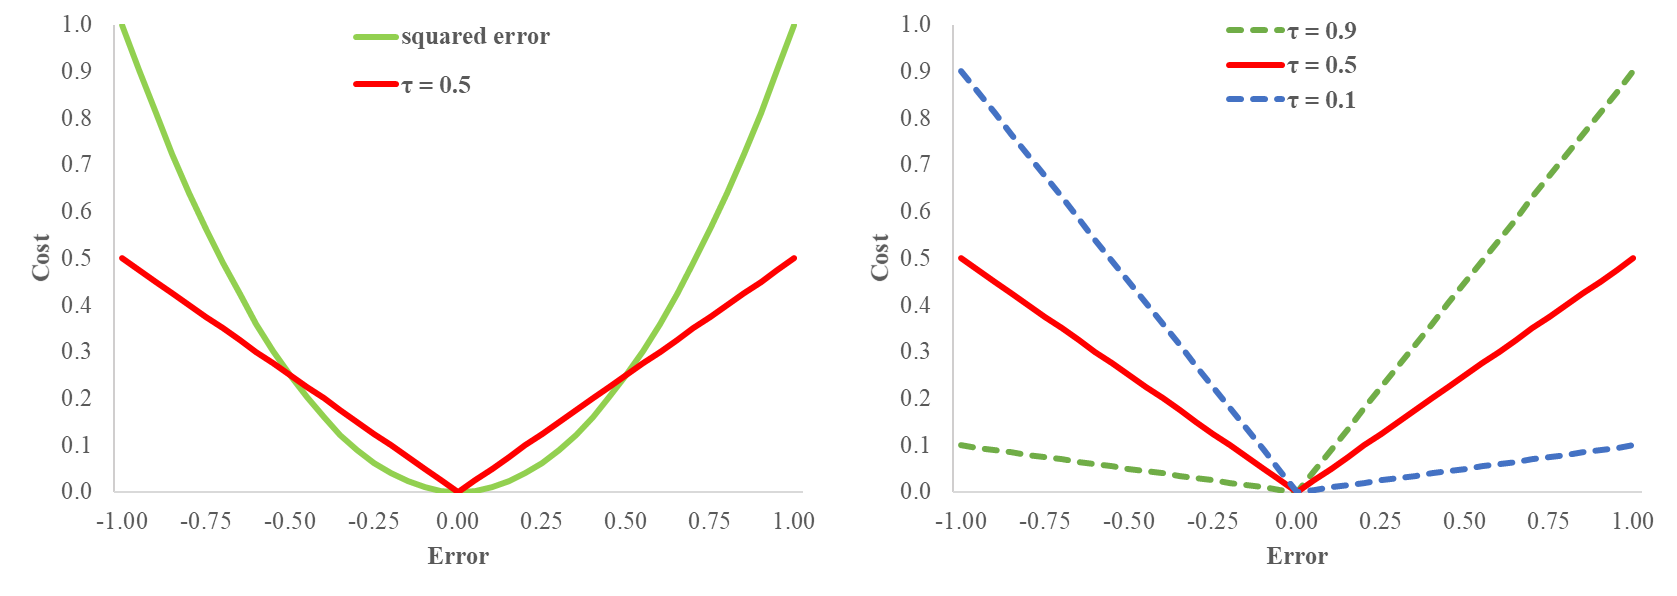
\includegraphics[width=0.75\linewidth]{Figures/quantile_reg_v2}
 \end{figure}

\end{frame}


\frame{
\frametitle{Trick is to Redefine the Residual Term}
  \vspace{0.25cm}
  \begin{itemize}
    \item Define $\epsilon_t = y_t - x_t\theta_t = u_t - v_t$, where
    \begin{eqnarray*}
    % \nonumber to remove numbering (before each equation)
      u_t &=& \mathbbm{1}_{(\epsilon_t \geq 0)} |\epsilon_t|\geq 0, \\
      v_t &=& \mathbbm{1}_{(\epsilon_t < 0)} |\epsilon_t|\geq 0. \\
    \end{eqnarray*}
  \item Minimization problem becomes
    \begin{equation*}
 \min_{\theta_{\tau} \in \mathbb{R}^K} \sum_{t=1}^{T} \left(\tau u_t + (1-\tau) v_t \right),
\end{equation*}
where the residuals must satisfy the $T$ constraints that
    \begin{equation*}
 y_t - x_t\theta = \epsilon_t = u_t - v_t.
\end{equation*}


  \end{itemize}

}


\frame{
\frametitle{Deriving the Linear Program}
  \vspace{0.25cm}
  \begin{itemize}
    \item This results in the linear program

    \begin{align*}
    &\min_{\theta_{\tau} \in \mathbb{R}^K, u \in \mathbb{R}^T, v \in \mathbb{R}^T} \sum_{t=1}^{T} \left\{\tau u_t +(1-\tau) v_t \right\}&\\
    s.t.\\
    &y_t - x_t\theta = u_t - v_t& \\
    &u_t \geq 0& \\
    &v_t \geq 0& \\
    \end{align*}
    which can be solved by interior point methods, among others.
    \bigskip
    \item[] \hyperlink{qr}{\beamerbutton{Back}}  

\end{itemize}


}

\subsection{Obtaining the Time Series of Conditional Quantiles}
\begin{frame}[noframenumbering]
\thispagestyle{empty}
       \begin{center}
         \structure{\Huge {\color{black}{\insertsubsection}}}
       \end{center}
     \end{frame}

\frame{
\frametitle{Obtaining the Time Series of Conditional Quantiles}
\framesubtitle{From 'Growth At Risk Models for the U.S. and the Foreign Economy (2020)'}
\label{TSQSteps}
\begin{itemize}
%   \item \textbf{Parametric assumptions} on the relationship between quantiles and conditioning variables:
% \begin{equation*}
%   \hat{\text{Q}}_{\tau} (\Delta \bar{y}_{t+1,t+12}| x_t) = \hat{\alpha}_{\tau} + \hat{\beta}_{\tau} VXO_t + \hat{\gamma}_{\tau} ADS_t,\ \tau \in (0,1).
% \end{equation*}
% \smallskip
%   \item Using data on $\Delta \bar{y}_{t+1,t+12}$ and $x_t$ we can estimate quantile regression slopes $\{\hat{\alpha}_{\tau},\hat{\beta}_{\tau},\hat{\gamma}_{\tau}\},\ \tau \in (0,1)$.
% \bigskip
\item At each point in time $t$, it is possible to use data on $VXO_t$ and $ADS_t$ to construct $\hat{\text{Q}}_{\tau} (\Delta \bar{y}_{t+1,t+12}| x_t)$.
\bigskip
\item \rr{Example}: March 2020, $VXO=63.32$; $ADS-6.42$.
  \bigskip
  \item Coefficients for the $10th$ quantile are
  \begin{equation*}
    \hat{\alpha}_{\tau=0.1} = -1.48,\ \hat{\beta}_{\tau=0.1} = -0.03,\ \hat{\gamma}_{\tau=0.1} = 1.53
  \end{equation*}
  \item $10th$ Conditional quantile is: 
  \bigskip
  {\footnotesize
    \begin{equation*}
    \hat{\text{Q}}_{\tau=0.1} (\Delta \bar{y}_{20:m4,\ 21:m3}| x_{20:m3}) = -1.48 + (-0.03) \cdot 63.32 + 1.53\cdot (-6.42) + \underbrace{2.37}_{trend} = -10.83
    \end{equation*}
    }
    \medskip
  \item Construct similarly remaining  quantiles ($25th$, $50th$, $75th$, $90th$).\\[0.25cm] \hyperlink{linearqr}{\beamerbutton{Back}}
% \bigskip
% \item Important: $\hat{\text{Q}}_{\tau} (\Delta \bar{y}_{t+1,t+12}| x_t)$ is an \textbf{output} of the model.
\end{itemize}

}


\subsection{Assessing Statistical Significance}
\begin{frame}[noframenumbering]
\thispagestyle{empty}
       \begin{center}
         \structure{\Huge {\color{black}{\insertsubsection}}}
       \end{center}
     \end{frame}



\frame{
\frametitle{Bootstrapping Techniques for Quantile Regressions}
\label{bootstrap}
\begin{itemize}
  \item \textbf{``Blocks-of-blocks''} bootstrap:
\medskip
\begin{enumerate}
  \item Divide the dependent variable $y$ and the regressors $X$ into $l$ consecutive blocks of all possible $m$-tuples.
  \medskip
  \item At each bootstrap replication, blocks of data are randomly drawn to form a new sample of the same size as the original data.
  \medskip
  \item Blocks are resampled in the same order for both the dependent variable $y$ and the regressors $X$, a key step which preserves the time-dependency in the data.
\end{enumerate}
\bigskip

\item Confidence intervals of bootstrapped coefficients' statistic $f(\beta_{b})$:
\medskip
\begin{enumerate}
  \item Generate statistic $f(\beta_{b})$ for each $b=1,\ldots,N_b$ bootstrap replicas.
  \medskip
  \item Construct percentiles of $f(\beta_{b})$ to obtain confidence interval.
\end{enumerate}
\end{itemize}

}


\frame{
\frametitle{``Blocks-of-Blocks'' Bootstrap Advantages}

\begin{itemize}
\item  Preserves crucial feature of quantile regression:\\ Agnostic about the underlying distribution of the error terms.
\bigskip
\item Maintains (time-series) dependency in the data, which would in most cases be destroyed by a naive bootstrap.
\bigskip
\item Used when a researcher is interested in computing confidence intervals around nonsymmetric statistics of the underlying data.
\bigskip
\item Relevant since our quantile regression model is a $h$-step predictive regression and slopes are non-linear functions of the data.
\bigskip
\item  See Chapter 12 of \citet{LutzHelmut2018} for more details.
\bigskip
\item[] \hyperlink{bootfullsample}{\beamerbutton{Back}}
\end{itemize}

}


\frame{
\frametitle{Conditional Quantiles over Time}
\framesubtitle{Global Financial Crisis}
\label{bootGFC}

\begin{figure}[!htb]
 \centering
 \includegraphics[width=\textwidth]{Figures/quantiles_bootstrap_GR}
\end{figure}
\medskip
\hyperlink{bootfullsample}{\beamerbutton{Back}}
}



\frame{
\frametitle{Conditional Quantiles over Time}
\framesubtitle{COVID-19 Outbreak}
\label{bootCOVID}

\begin{figure}[!htb]
 \centering
 \includegraphics[width=\textwidth]{Figures/quantiles_bootstrap_recent}
\end{figure}
\medskip
\hyperlink{bootfullsample}{\beamerbutton{Back}}
}



\subsection{From Quantiles to Distributions\\ \bigskip \large A Step-by-Step Example}
\begin{frame}[noframenumbering]
\thispagestyle{empty}
       \begin{center}
         \structure{\Huge {\color{black}{\insertsubsection}}}
       \end{center}
     \end{frame}


\frame{
\frametitle{A Step-by-Step Example\\ \small Fitting the Skewed $t$-Distribution}
 {
 \label{azzsbs}
\begin{itemize}
  \item In March 2020, the four quantiles to fit the distribution are:
  \begin{eqnarray*}
    \hat{\text{Q}}_{\tau=0.10} (\Delta \bar{y}_{20:m4,\ 21:m3}| x_{20:m3}) &= -10.83,  &CI_{90\%}=[-14.53,-7.21]\\
    \hat{\text{Q}}_{\tau=0.25} (\Delta \bar{y}_{20:m4,\ 21:m3}| x_{20:m3}) &= -\phantom{1}5.51,  &CI_{90\%}=[-8.05,-3.11]\\
    \hat{\text{Q}}_{\tau=0.75} (\Delta \bar{y}_{20:m4,\ 21:m3}| x_{20:m3}) &=  \phantom{-1} 0.08,  &CI_{90\%}=[-1.49,0.83]\\
    \hat{\text{Q}}_{\tau=0.90} (\Delta \bar{y}_{20:m4,\ 21:m3}| x_{20:m3}) &= \phantom{-1} 0.37, &CI_{90\%}=[-0.98,1.52]\\
  \end{eqnarray*}
  \item
  Find distribution parameters ${\Theta}$ that minimize distance between:
  \begin{center}
      $\hat{\text{Q}}_{\tau=\{0.1,0.25,0.75,0.9\}}(\Delta \bar{y}_{20:m4,\ 21:m3}| x_{20:m3})$ from QR model and\\
  $F^{-1}_{\Delta \bar{y}}(\tau=\{0.1,0.25,0.75,0.9\}|x_{20:m3},{\Theta})$ from skewed $t-$distribution.
  \end{center}
  \bigskip
\item Density in March 2020 is skewed $t$-PDF $\ f(\Delta \bar{y}_{20:m4,\ 21:m3}|x_{20:m3},\hat{\Theta})$ constructed using estimated distribution parameters $\hat{\Theta}$.
\end{itemize}
\smallskip
\hyperlink{azzintro}{\beamerbutton{Back}}
}}


\subsection{Assessing the Correct Calibration of the Model}
\begin{frame}[noframenumbering,label={PITs}]
\thispagestyle{empty}
       \begin{center}
         \structure{\Huge {\color{black}{\insertsubsection}}}
       \end{center}
     \end{frame}


\frame{
\frametitle{A Formal Test\\ \small \cite{RossiSekhposyan2019}}

\begin{itemize}
  \item Test for correct calibration of the conditional predictive distributions implied by the quantile regression model.
  \bigskip
  \item \bb{Correct calibration}: Probability that the realized value is above or below the predicted value is the same (on average, across time) irrespectively of whether realizations are high or low.
  \bigskip
  \item The test evaluates the absolute predictive ability of a model at its estimated parameter values and, thus, in finite samples.
      \bigskip
  \item In this sense, both the parametric model and the estimation technique employed are being evaluated.
\end{itemize}

}


\frame{
\frametitle{How the Tests Works in Practice}

\begin{itemize}
\item Estimate the quantile regression model and construct out-of-sample conditional quantiles.
\medskip
\item Fit distribution on out-of-sample conditional quantiles.
\medskip
\item Back out quantile of realized value from predicted distribution, formally known as the probability integral transform (PIT):
    \begin{equation*}
    PIT_t \equiv Prob\left(\Delta \bar{y}_{t+1,t+12}<\Delta \bar{y}^*_{t+1,t+12}|x_t\right).
    \end{equation*}

\medskip

\item In a perfectly calibrated model, the predictive density should feature a CDF which is uniform, i.e., equal to the $45^{\circ}$ line.

\medskip

\item If the empirical CDF of the PITs falls outside of the 5\% critical values, the null hypothesis of correct calibration is rejected.
\end{itemize}

}



\frame{
\frametitle{Evaluating Correct Calibration of Our Model}

\begin{figure}[!htb]
 \centering
 \includegraphics[width=0.7\textwidth]{Figures/RS_OOS____Country=US___GDP=GDP___SpecWith=vix_ads___Scenario=Baseline___Lags=0___Detrended=true___Sample=1986-Jan_to_2020-Mar}
\end{figure}

}


\frame{
\frametitle{Comparison to \citet{Adrianetal2019}}

\begin{figure}[!htb]
 \centering
 \includegraphics[width=0.7\textwidth]{Figures/RS_OOS____Country=US___GDP=GDPG___Scenario=Baseline___Lags=0___Detrended=false___Sample=1986-Q1_to_2019-Q4}\\
 {\scriptsize{Note: For comparison purposes, our model has been adapted to quarterly frequency.}}
\end{figure}
\hyperlink{azzintro}{\beamerbutton{Back}}
}


\subsection{Data \& Estimation}
\begin{frame}[noframenumbering,label={Data}]
\thispagestyle{empty}
       \begin{center}
         \structure{\Huge {\color{black}{\insertsubsection}}}
       \end{center}
     \end{frame}
     
\frame{
\frametitle{Data \& Estimation}
\framesubtitle{From 'Growth At Risk Models for the U.S. and the Foreign Economy (2020)'}

\begin{itemize}
    \item Average GDP growth between months $t+1$ and $t+12$
    \medskip
    \item CBOE S\&P100 Volatility Index (VXO)
    \medskip
    \item Arouba Diebold Scotti country-specific indexes estimated using a dynamic factor model with mixed frequency data:
    \smallskip
\begin{itemize}
    \item Annualized quarterly growth rates of {\rr{real GDP}};
    \smallskip
    \item Annualized monthly growth rates of retail sales;
    \smallskip
    \item Annualized monthly growth rates of industrial production;
    \smallskip
    \item The new export order component of the PMI survey;
    \smallskip
    \item Initial unemployment insurance claims (United States ADS only)
\end{itemize}
\medskip
\item {\rr{Estimation Sample}}: 1986:m1 - 2019:m3.\\
$\longrightarrow$ Last in-sample observation of future GDP growth in 2019:m3 based on data from 2019:m4 through 2020:m3.
\end{itemize}

\vspace*{0.2in}
\hyperlink{linearqr}{\beamerbutton{Back}}
}


\subsection{Alternative Financial Indicators}
\begin{frame}[noframenumbering,label={alterfin}]
\thispagestyle{empty}
       \begin{center}
         \structure{\Huge {\color{black}{\insertsubsection}}}
       \end{center}
     \end{frame}

\frame{
\frametitle{Quantile Estimates: Alternative Financial Indicators}
%\framesubtitle{From \citet{Adrianetal2019}}
\label{qr-estimates-abg}

% \begin{figure}[!htb]
%  \centering
%  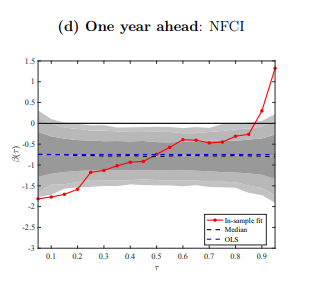
\includegraphics[width=0.5\textwidth]{Figures/abgqrnfci.png}
% \end{figure}
\begin{figure}[!htb]
 \centering
 {\scriptsize{NFCI and GDP growth  (Adrian et al., 2019)}}\\
 \includegraphics[width=0.38\textwidth]{Figures/slope_nfci___Country=US___GDP=GDPG___SpecWith=gdp_nfci___Scenario=Baseline___Lags=0___Sample=1973-Q1_to_2015-Q4.pdf} \includegraphics[width=0.38\textwidth]{Figures/slope_gdp___Country=US___GDP=GDPG___SpecWith=gdp_nfci___Scenario=Baseline___Lags=0___Sample=1973-Q1_to_2015-Q4.pdf}

 
\end{figure}

\begin{figure}[!htb]
 \centering
 {\scriptsize{BAA-10-Year spread and GDP growth}}\\
 \includegraphics[width=0.38\textwidth]{Figures/slope_baa10ym___Country=US___GDP=GDPG___SpecWith=gdp_baa10ym___Scenario=Baseline___Lags=0___Sample=1973-Q1_to_2015-Q4.pdf} \includegraphics[width=0.38\textwidth]{Figures/slope_gdp___Country=US___GDP=GDPG___SpecWith=gdp_baa10ym___Scenario=Baseline___Lags=0___Sample=1973-Q1_to_2015-Q4.pdf}

\end{figure}
\vspace*{-0.2in}
\hyperlink{disadvantagesqr}{\beamerbutton{Back}}

}


\subsection{Approximation Error}
\begin{frame}[noframenumbering,label={approxerrorabg}]
\thispagestyle{empty}
       \begin{center}
         \structure{\Huge {\color{black}{\insertsubsection}}}
       \end{center}
     \end{frame}

\frame{
\frametitle{Estimating PDFs from QR: Approximation Error}
\framesubtitle{From \citet{Adrianetal2019}}
\label{approxerrprabg}

\begin{figure}[!htb]
 \centering
 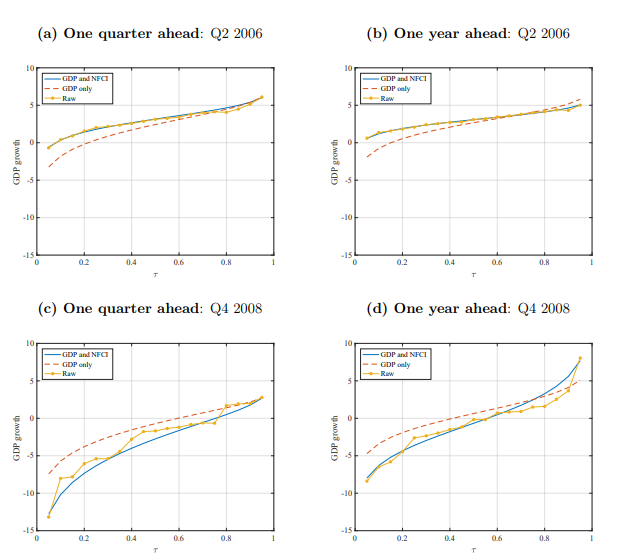
\includegraphics[width=0.67\textwidth]{Figures/approxerrorABG.png}
\end{figure}

\vspace*{-0.2in}
\hyperlink{azzintro}{\beamerbutton{Back}}

}



\frame{
\frametitle{References}
\bibliographystyle{chicago}
\bibliography{qr}
}







\end{document}
